\documentclass[10pt]{beamer}
\usetheme{Pittsburgh}

\usepackage{graphicx}
\usepackage[linesnumbered,ruled,vlined]{algorithm2e}
\usepackage{color,soul}
\usepackage[utf8]{inputenc}
\usepackage[T1]{fontenc}
\usepackage{textcomp}
\usepackage{amsmath, amssymb}
\usepackage{caption}
\usepackage{listings}
\usepackage[italian]{babel}

% figure support
\usepackage{tikz}
\usetikzlibrary{calc}
\usepackage{import}
\usepackage{xifthen}
\usepackage{pdfpages}
\usepackage{transparent}
\usepackage[]{hyperref}
\usepackage{multirow}

% provides the H option
\usepackage{float}

% provides subcaptions
\usepackage{subcaption}

% provides justification
\usepackage{ragged2e}
\justifying

% for logo
\usepackage[export]{adjustbox}

\pdfsuppresswarningpagegroup=1
\setcounter{tocdepth}{1}
\AtBeginSection[]
{
  \begin{frame}<beamer>
    \tableofcontents[currentsection,depth=1]
  \end{frame}
}

\author{Augello Andrea \and Castiglione Francesco Paolo \and La Martina Marco}
\institute{Università degli studi di Palermo}
\begin{document}
\title[Chang'e]{Documentazione - Progetto di Robotica}
	\begin{frame}
		\titlepage
		\begin{figure}[htpb]
			
\includegraphics[width=0.2\textwidth,left]{./img/logo_unipa.png}
		\end{figure}
		
		
	\end{frame}


	\section{Introduzione}\label{sec:Introduzione}
	\frame{\sectionpage}
	\frame{
		La pandemia del coronavirus SARS-CoV-2 ha dato una forte
		spinta alla ricerca sia nel campo sanitario che informatico, mettendo in
		evidenza forti carenze dal punto di vista infrastrutturale.
		
		
		Al momento, considerando la limitata disponibilità del vaccino alle masse, uno dei miglior modi di evitare la contrazione del coronavirus è
		di evitarne l'esposizione. Il distanziamento sociale si configura di
		conseguenza come un prerequisito per una significativa riduzione del numero
		di infetti, come evidenziato da simulazioni di un sistema ad agenti
		\cite{silva2020covid}. Un problema chiave si configura di conseguenza come
		il controllo del rispetto delle norme di distanziamento all'interno degli
		spazi chiusi. 
	}

	\begin{frame}{Obbiettivo}
	L'obbiettivo del progetto è quello di sviluppare un robot con lo scopo di \textbf{evitare assembramenti in ambienti indoor} e di invitare a \textbf{rispettare le norme sul distanziamento sociale}. 
	
	Nella dimostrazione presentata il nostro robot rileva le persone nella stanza e individua i possibili assembramenti. In seguito alla fase di rilevazione si sposterà verso l'assembramento evitando gli ostacoli e, arrivato, esorterà le persone al rispetto del distanziamento sociale.
	\end{frame}
	
	\begin{frame}{Stato dell'arte}
	Un robot che si occupa di far rispettare il distanziamento sociale è quello
	proposto nell'articolo~\cite{sathyamoorthy2020covidrobot}. Sono stati usati
	un TurtleBot 2, una camera RGB-D e CCTV per il rilevamento degli
	assembramenti, una camera termica per rilevare la temperatura corporea e un
	lidar 2-D per evitare le collisioni.
	
	Un altro esempio è quello proposto nell'articolo~\cite{fan2020autonomous}.
	In questo caso sono state usate 2 camere e CCTV per il rilevamento degli
	assembramenti e un lidar 3-D per evitare le collisioni.
	
	\begin{figure}[H]
		\begin{subfigure}{0.49\textwidth}
			\centering
			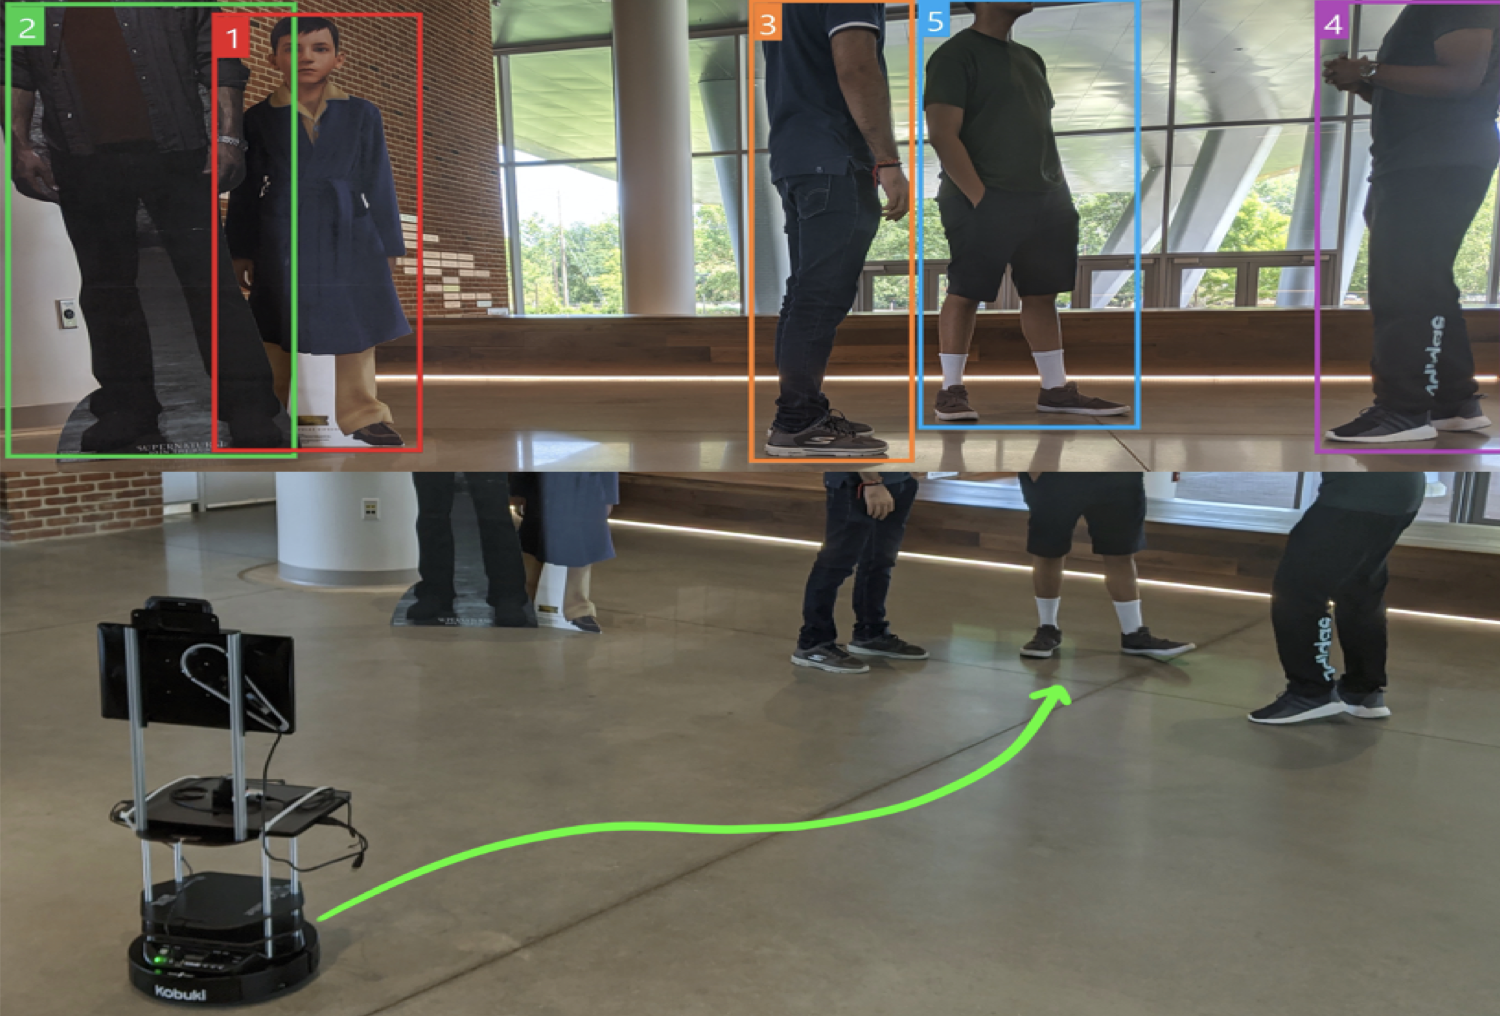
\includegraphics[width=0.8\linewidth]{./img/State_of_art_1.png}
		\end{subfigure}
		\begin{subfigure}{0.49\textwidth}
			\centering
			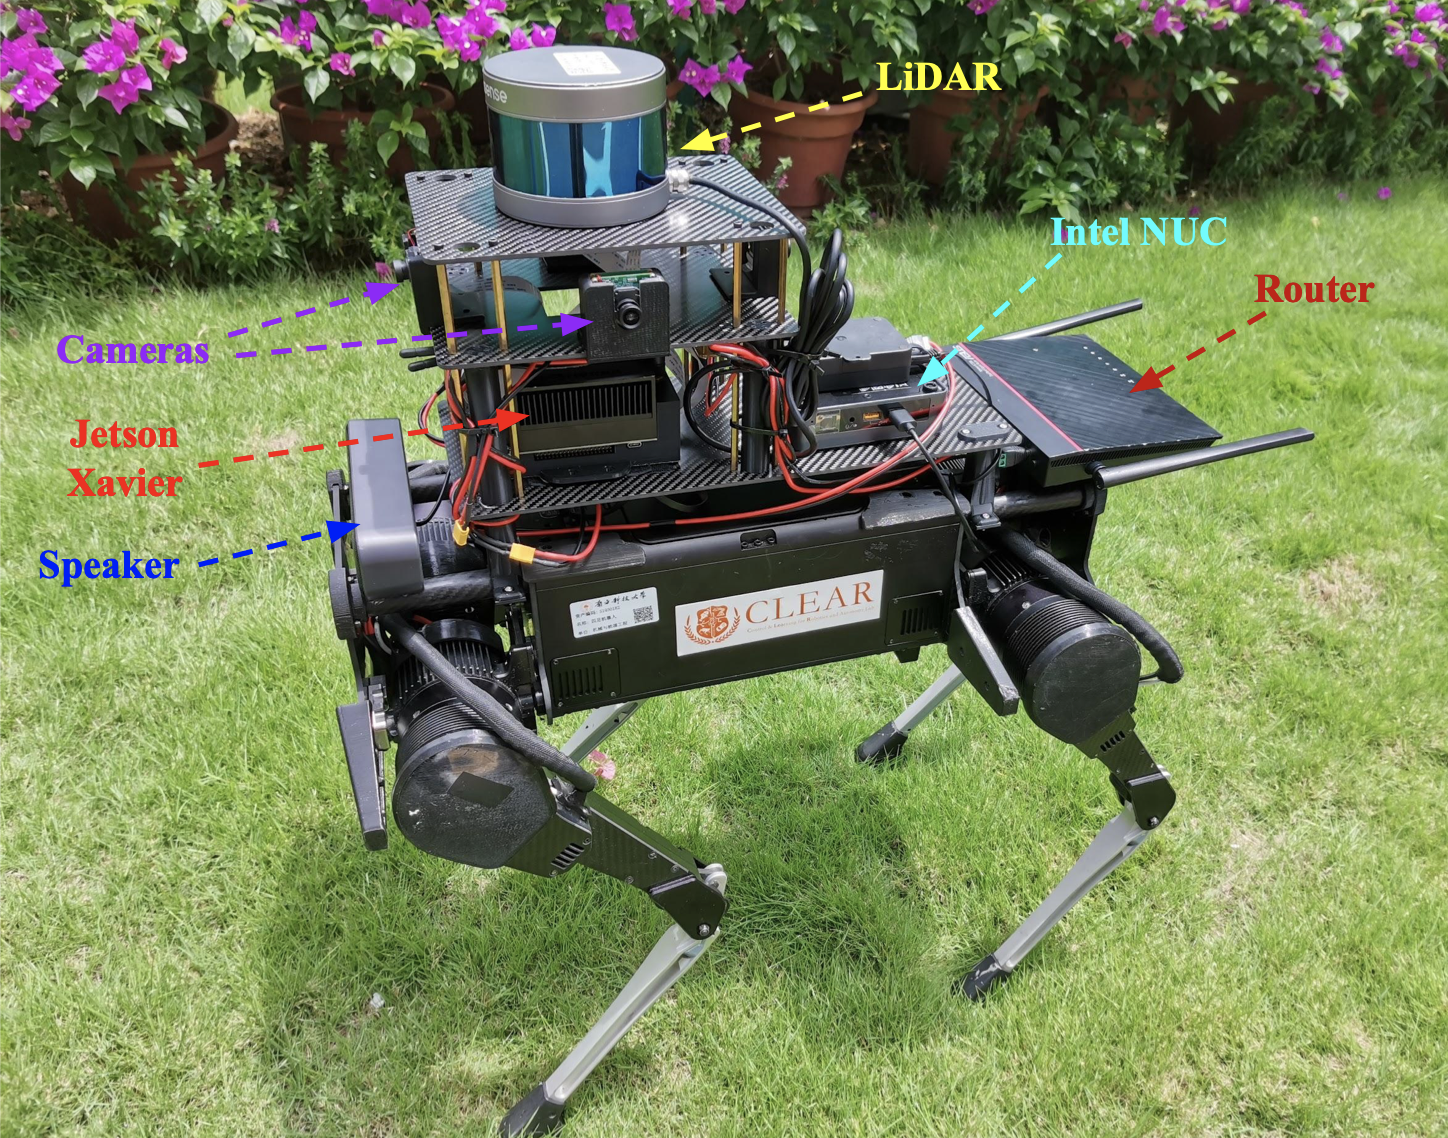
\includegraphics[width=0.8\linewidth]{./img/State_of_art_2.png}
		\end{subfigure}
	\end{figure}
	
	\end{frame}
	
	\begin{frame}{Setup}
	\centering
	\begin{tabular}{|l|l|}
		\hline
		\multirow{2}{4em}{OS} & Ubuntu 18.04 \\
							  & Ubuntu 20.04 \\ \hline
		\multirow{2}{6em}{ROS version} & melodic \\
									   & noetic \\ \hline
		Webots	& R2020b revision 1\\ \hline
		OpenCV~\cite{opencv} 	& 4.x \\\hline
		Imutils~\cite{imutils} & 0.5.3 \\\hline
		Matplotlib~\cite{matplotlib} & 3.3.3 \\\hline
		Numpy~\cite{numpy} & 1.17.2 \\\hline
		Scikit-learn~\cite{scikit} & 0.21.3\\\hline
		{Target hardware}  & Raspberry Pi 3B+ \\ \hline
	\end{tabular}
	\end{frame}


	\section{Gestione dei nodi ROS}\label{sec:Ros}
	\frame{\sectionpage}

	\frame{\begin{figure}[H]
		\centering
		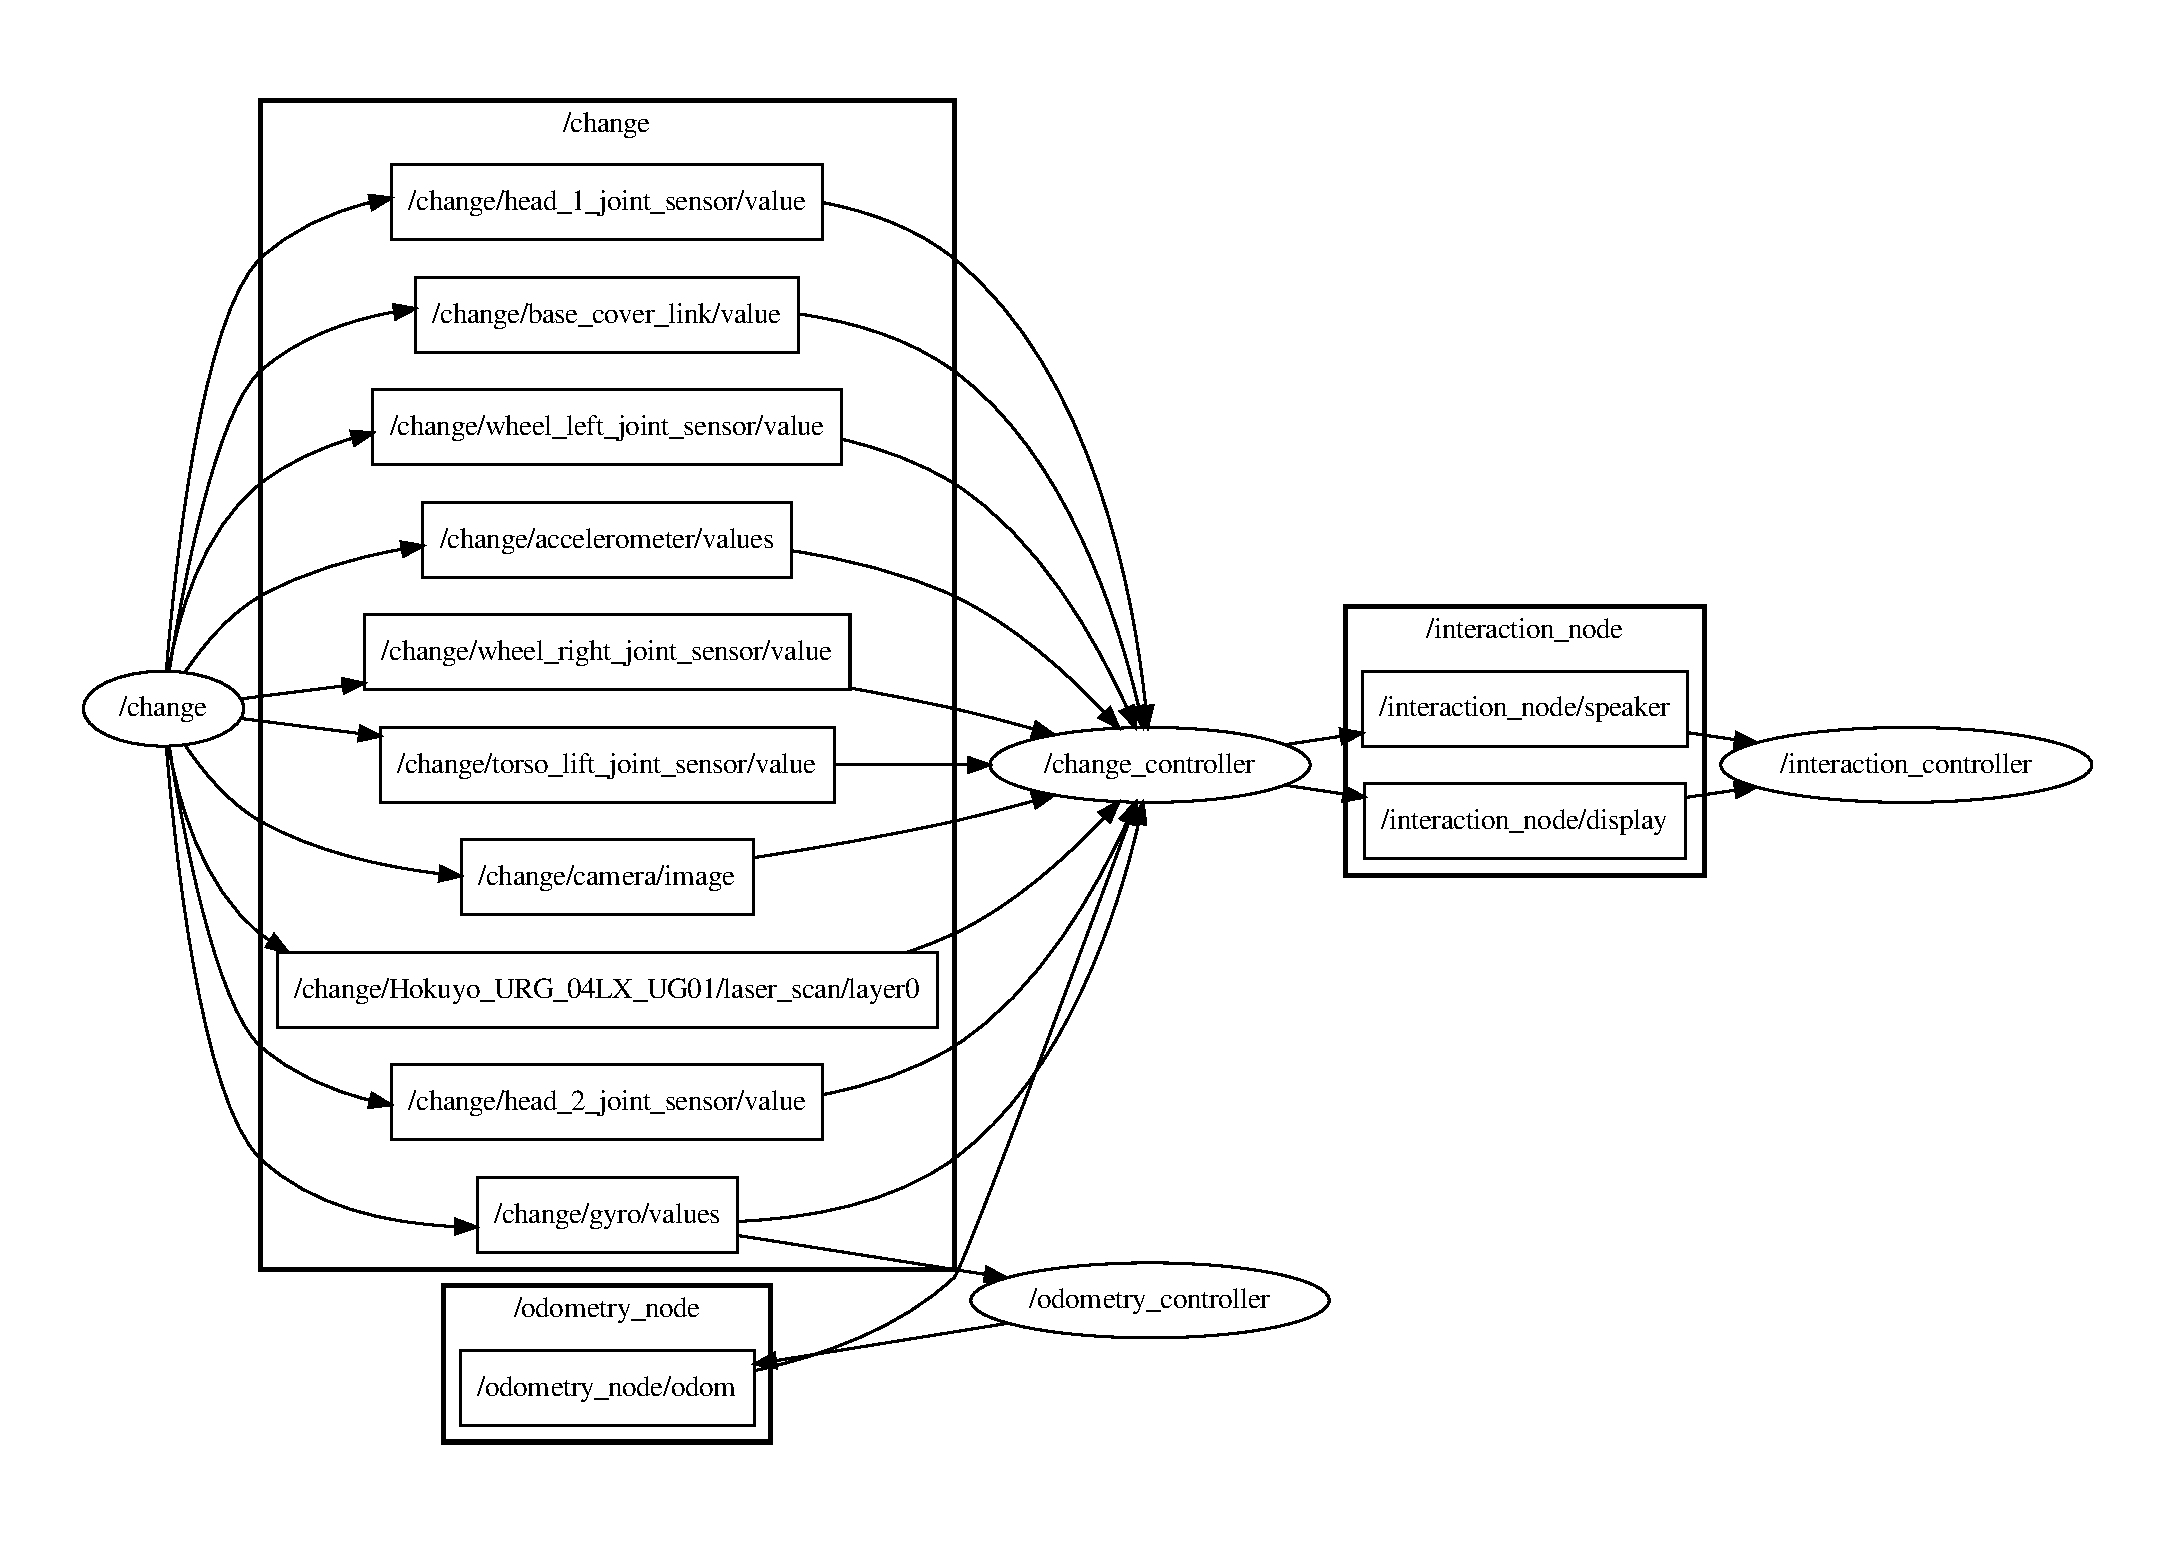
\includegraphics[width=1\textwidth]{img/rosgraph.pdf}
		\caption{Architettura dei nodi ros, ottenuta tramite \textit{rqt}}
		\label{fig:rosgraph}
	\end{figure}
	}

	\begin{frame}{Webots node}
	Questo nodo si occupa solamente di lanciare Webots, e di impostare il
	valore del clock di ROS in base al tempo della simulazione, in modo da
	potere effettuare le integrazioni del tempo correttamente.
	\end{frame}
	\begin{frame}{Change controller node}
	Questo è il nodo che si occupa della gran parte della elaborazione. Oltre
	ad arbitrare sui comportamenti da assumere, gestisce più moduli che si
	occupano di: 
	\begin{itemize}
		\item acquisire i dati dai sensori
		\item mandare i comandi ai motori
		\item gestire il movimento, quindi rotazioni e traslazioni
		\item acquisire e analizzare le immagini dalla camera
	\end{itemize}
	\end{frame}

	\begin{frame}{Interaction node}
	Questo nodo ha il compito di gestire le interazioni audio/video. Ogni
	messaggio che viene riprodotto, prima in lingua italiana e poi inglese,
	viene anche visualizzato testualmente sullo schermo in italiano, inglese e
	cinese.  I possibili comportamenti assunti dal robot sono:
	\begin{itemize}
		\item Salutare all'avvio
		\item Mostrare sul display immagini che esortano a rispettare il
			distanziamento sociale
		\item Riprodurre un messaggio audio che invita a rispettare il distanziamento sociale quando
			rileva un assembramento o quando scansiona l'ambiente
	\end{itemize}
	\end{frame}

	\begin{frame}{Odometry node}
	Il nodo che si occupa dell'odometria si occupa di stimare la posizione del
	robot, come spiegato approfonditamente nella
	sezione~\ref{sec:Modello-del-moto-e-posizionamento}. In generale ciò che fa
	è integrare costantemente i valori del giroscopio e della velocità delle
	ruote per condividere posizione e orientamento del robot.
	\end{frame}
	
	
	\section{TIAGo Iron}\label{sec:TIAGo-Iron} 
	\frame{\sectionpage}
	\frame{

	\begin{columns}
		\begin{column}{0.7\textwidth}
		\justifying
		Il robot scelto per l'obbiettivo proposto è il \textbf{TIAGo Iron}, un
		robot umanoide a due ruote con torso e testa ma senza braccia articolate \cite{pages2016tiago}.
		
		Il datasheet del \textbf{TIAGo} \cite{tiago_datasheet} indica la presenza di speaker e display, non  presenti nel modello Webots \cite{tiagoiron}, che sono quindi stati aggiunti.
		
		La camera del \textbf{TIAGo} è RGB-D ma il modello Webots ne è sprovvisto, di conseguenza è stata utilizzata una camera monoscopica RGB. 
		
		L'IMU utilizzata ha 6 gradi di libertà. 
		
		Il modello Webots del \textbf{TIAGo} presenta un lidar (Hokuyo URG-04LX-UG01 \cite{lidarspecs}) che, conformemente al datasheet,  ha un range di $5.6\,m$ ed un FOV di $240^{\circ}$ (agli estremi è parzialmente occluso).
		\end{column}
		
		\begin{column}{0.3\textwidth}
			\begin{figure}[htpb]
				\centering
				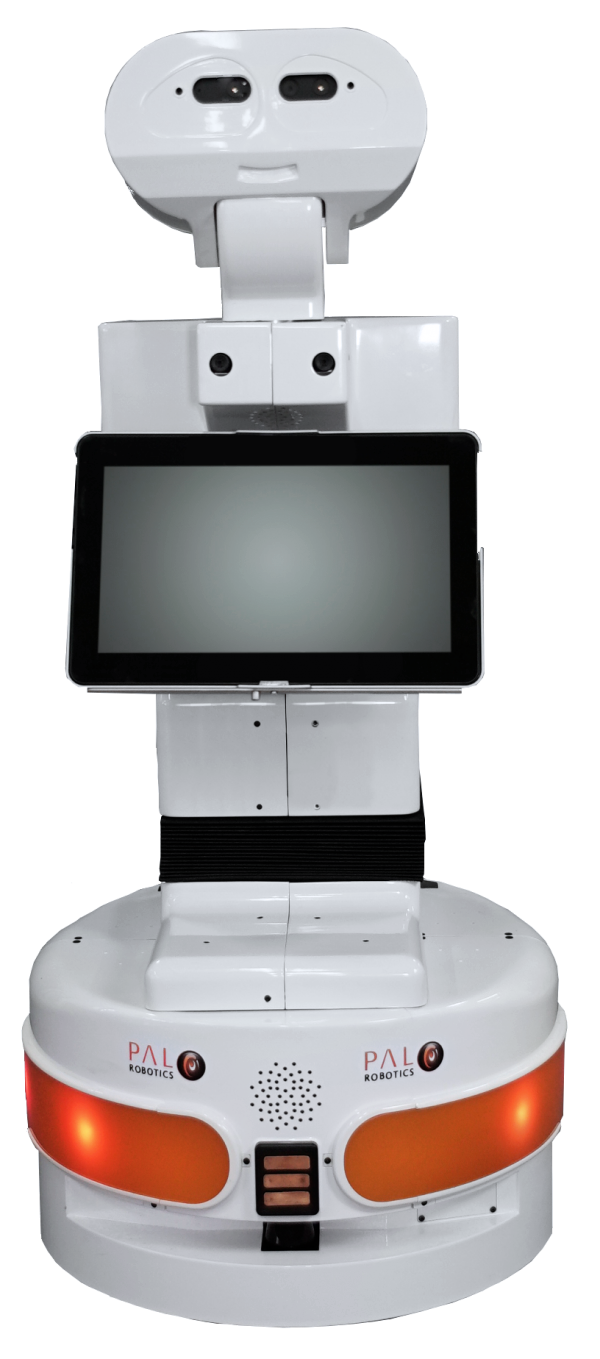
\includegraphics[width=\textwidth]{./img/tiago.png}
				\label{fig:tiago}
			\end{figure}
		\end{column}
	\end{columns}
	
	}

	\section{Modello del moto e posizionamento}\label{sec:Modello-del-moto-e-posizionamento} 
	\frame{\sectionpage}
	
	\begin{frame}{Orientamento}
		Il modello del moto è caratterizzato da rotazioni e traslazioni. Per le
		rotazioni ci basiamo sui dati forniti dal giroscopio, il quale fornisce
		una velocità angolare. Calcoliamo quindi l'angolo di rotazione
		effettuando un'integrazione discreta dei campioni con interpolazione
		lineare del primo ordine (Eq.~\ref{eq:gyro-integration}).  
		\begin{equation}\label{eq:gyro-integration}
			\theta_i = \sum_{j=1}^i \frac{\omega _{j-1}+\omega _j}{2} \left( t_j-t_{j-1} \right) 
		\end{equation}
		Noto l'angolo corrente e l'angolo target utilizziamo un controllore
		proporzionale per raggiungere l'angolo desiderato.
	\end{frame}
	
	\begin{frame}{Spostamento}
		Per effettuare lo spostamento lineare utilizziamo il controllore PID
		
		(Proporzionale-Integrale-Derivativo) delle ruote fornito da Webots, che
		richiede un angolo di rotazione target per ogni ruota. Utilizziamo quindi
		l'angolo di rotazione corrente, e il diametro delle ruote per calcolare la
		posizione delle ruote necessaria al fine di ottenere lo spostamento
		desiderato (Eq.~\ref{eq:odometry}).
		\begin{equation}\label{eq:odometry}
		targetAngle =
		currentAngle+2\pi\frac    {distance}
						{2\pi \cdot diameter}
		\end{equation}
	\end{frame}
	
	\subsection{Posizionamento}\label{subsec:Posizionamento}
	\begin{frame}{Posizionamento}
		Inizialmente al segnale dell'accelerometro
		veniva applicato un integrale doppio per ottenere lo spostamento
		lineare(Eq.~\ref{eq:accel-integration} 	\cite{positioning}).
		
		\begin{equation}\label{eq:accel-integration}
			\begin{cases}
				\textbf{v}_i & = \sum_{j=1}^{i} \frac{\textbf{a} _{j-1}+\textbf{a} _j}{2} \left( t_j-t_{j-1} \right) \\
				\textbf{s}_i & = \sum_{j=1}^{i} \frac{\textbf{v} _{j-1}+\textbf{v} _j}{2} \left( t_j-t_{j-1} \right) 
			\end{cases}
		\end{equation}
		
		Abbiamo ritenuto necessario cambiare approccio, decidendo di utilizzare gli
		encoders delle ruote per determinare gli spostamenti. 
		
		Integriamo la velocità lineare del robot, calcolata a
		partire dal raggio R e le velocità angolari $u[t]$ delle ruote.
		
		\begin{equation}\label{eq:linear-velocity}
			v_i = \frac{R (u_{r,i}+u_{l,i})}{2}
		\end{equation}
		
		Questi valori sono aggiornati ad ogni intervallo di campionamento utilizzando la velocità lineare e la velocità angolare del robot \cite{572228}.
		
		\begin{equation}\label{eq:position-vector-update}
			\textbf{P}_i = \sum_{j = 1}^{i} \begin{bmatrix}
				 & v_i\cos(\theta_i ) & \\
				 & v_i\sin(\theta_i )
			\end{bmatrix}\cdot (t_j-t_{j-1}) 
		\end{equation}		
		
	\end{frame}
	\begin{frame}
		\begin{figure}[H]
			\begin{subfigure}{0.49\textwidth}
				\centering
				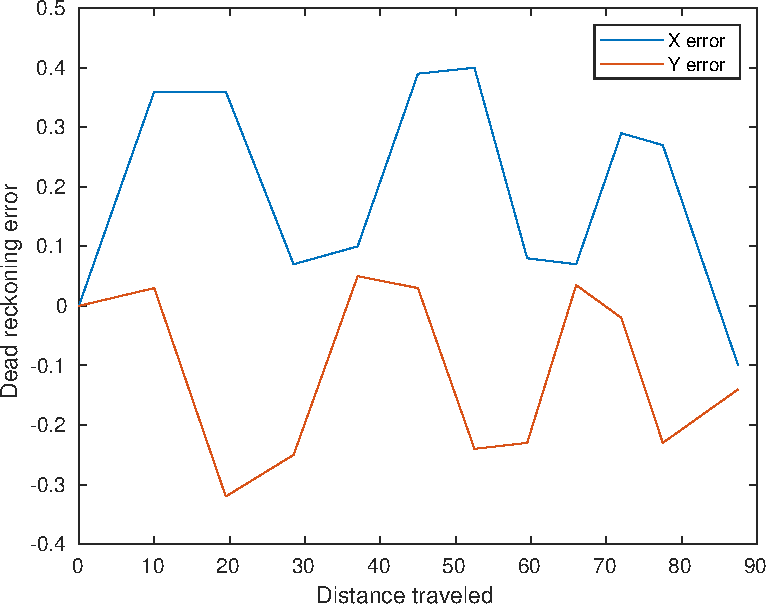
\includegraphics[width=0.8\linewidth]{./img/dead_reckoning_error.pdf}
				\caption{Errore nella stima della posizione}
				\label{fig:dead_reckoning_error}
			\end{subfigure}
			\begin{subfigure}{0.49\textwidth}
				\centering
				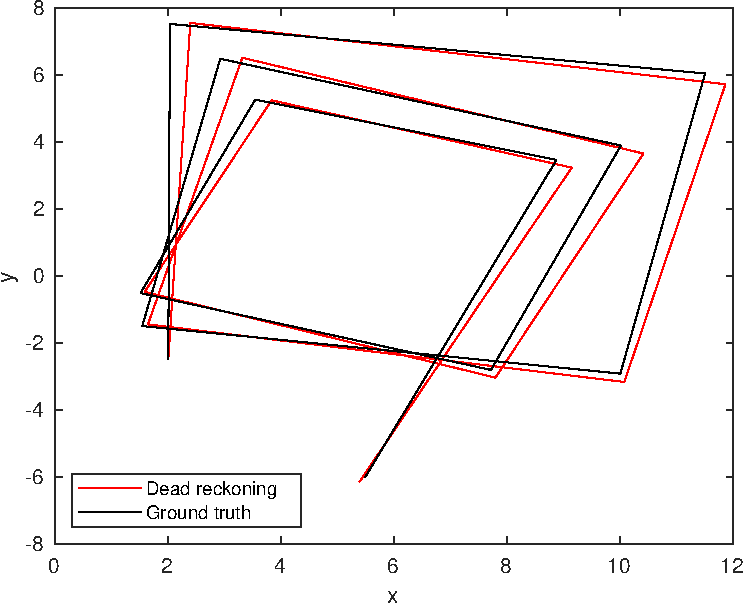
\includegraphics[width=0.8\linewidth]{./img/trajectories.pdf}
				\caption{Errore nella stima della traiettoria}
				\label{fig:trajectory_error}
			\end{subfigure}
		\end{figure}

		Abbiamo misurato le performance della stima di posizione e i risultati
		sono ritenuti soddisfacenti per raggiungere l'obbiettivo proposto.
	\end{frame}
	
	\begin{frame}{Collision avoidance}
		Il \textbf{TIAGo} è in grado di rilevare gli ostacoli grazie
		all'utilizzo di un sensore lidar.  
		
		Nell'immagine seguente viene mostrata la zona nella quale, se viene
		indicata dal lidar la presenza di un ostacolo, il \textbf{TIAGo} si
		ferma per ragioni di sicurezza al fine di evitare danni a persone e/o
		oggetti.
		\begin{figure}[H]
			\centering
			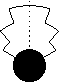
\includegraphics[width=0.2\textwidth]{./img/collision_avoidance.pdf}
			\caption{Collision avoidance}
			\label{fig:collision_avoidance}
		\end{figure}
	\end{frame}
	
	\section{Object recognition}\label{sec:Object-recognition}
	\frame{\sectionpage}
	
	\begin{frame}{Campionamento delle immagini}
		Il FOV della camera è di 57°, quindi per ricoprire 360° è necessario
		effettuare 7 campionamenti. Il settimo campionamento, come si vede in
		figura \ref{fig:campionamento_immagini}, è sovrapposto al primo per 39°.

		È possibile che un individuo si trovi in una zona di confine
		tra due campioni, e che quindi non sia correttamente identificabile in
		nessuna delle due immagini in cui appare parzialmente. Mitighiamo
		questo problema effettuiamo una rudimentale operazione di image
		mosaicing~\cite{ghosh2016survey} e campioniamo l'immagine così
		ottenuta ad intervalli di 28°.
		
		
		\begin{figure}[H]
			\centering
			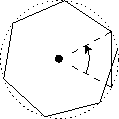
\includegraphics[width=0.3\textwidth]{./img/pictures_sampling.pdf}
			\caption{Campionamento delle immagini}
			\label{fig:campionamento_immagini}
		\end{figure}
	\end{frame}
	
	\begin{frame}{YOLO}
		Abbiamo valutato le performance di
		YOLOv3 (you only look once), YOLOv3-tiny, HoG (Histogram of oriented
		gradients), HoG + SVG (support vector machines).  In seguito a vari test su HoG abbiamo ritenuto essere
		problematica la larghezza delle bounding boxes fornite. YOLOv3 fornisce risultati soddisfacenti.
		
		Considerando le caratteristiche hardware del robot mobile, abbiamo optato per l'uso di
		YOLOv3-tiny, il quale risulta essere significativamente più efficiente
		(approssimativamente del 442\% \cite{tiny_yolo}). Inoltre è rilevante in tal senso un paragone fra YOLOv3 e
		YOLOv3-tiny in termini di mAP (mean average precision) e FLOPS
		(floating-point operations per second) addestrate sul dataset COCO, come
		illustrato dalla tabella.
		
		\begin{table}[htpb]
			\centering
			\begin{tabular}{ |c|c|c|c| } 
				\hline
				Model & mAP & FLOPS & FPS \\
				\hline	
				 YOLOv3-320    & 51.5  &  38.97  Bn  &  45  \\ 
				 YOLOv3-416    & 55.3  &  65.86  Bn  &  35  \\ 
				 YOLOv3-608    & 57.9  &  140.69 Bn  &  20  \\ 
				 YOLOv3-tiny   & 33.1  &  5.56   Bn  &  220 \\
				 YOLOv3-spp    & 60.6  &  141.45 Bn  &  20  \\
				\hline
			\end{tabular}
			\label{tab:comparison}
		\end{table}
		
	\end{frame}

	\section{Posizione dei target}\label{sec:Posizione-dei-target}
	\frame{\sectionpage}
	
	\subsection{Triangolazione}\label{subsec:Triangolazione}
	\begin{frame}{Triangolazione}
		\begin{columns}
			\begin{column}{0.6\textwidth}
				\justifying
				La triangolazione come metodo di individuazione delle persone
				presenta dei problemi nel nostro scenario:
				\begin{itemize}
					\justifying
					\item Occlusione delle persone: se due persone
						(5 e 2) sono una dietro l'altra lungo una retta
						immaginaria che le congiunge al robot (B), quest'ultimo
						non sarà in grado di individuare la più distante. 

					\item Imputazione delle osservazioni: quando il robot
						effettua scan successivi non è in grado di dedurre
						quali osservazioni derivano dalla stessa persona.
						Non è possibile determinare quali intersezioni
						corrispondono ad osservazioni reali e quali sono spurie. 

				\end{itemize}
			\end{column}
			
			\begin{column}{0.4\textwidth}
				\begin{figure}[htpb]
					\centering
					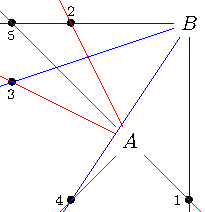
\includegraphics[width=\textwidth]{./img/ideal_object_triangulation.pdf}
					\label{fig:triangulation}
				\end{figure}
			\end{column}
		\end{columns}
	\end{frame}
	
	\subsection{Calcolo della distanza}\label{subsec:Calcolo-della-distanza}
	\begin{frame}[allowframebreaks]{Calcolo della distanza}
		Ipotizzando che la camera abbia un FOV (field of view) di
		$2\alpha$ e sia distante $d$ dall'oggetto, la massima distanza
		orizzontale che un punto dell'immagine potrebbe avere dal centro del
		piano dell'immagine sarebbe $a = d \tan \alpha$.
		
		\begin{figure}[H]
			\centering
			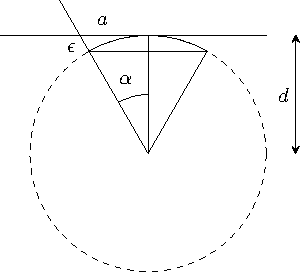
\includegraphics[width=0.4\textwidth]{./img/linearization_error.pdf}
		\end{figure}
		
		Ignorare la prospettiva significa effettuare un'approssimazione lineare
		del primo ordine e trattare il punto come se si trovasse su una
		circonferenza di raggio $d$ centrata sulla camera. Di conseguenza
		consideriamo il punto come se fosse più vicino di quanto non sia
		realmente, commettendo l'errore mostrato nell' Eq.~\ref{eq:max_err}.
		Con una camera con FOV di 1 radiante la sottostima è del 13.9\%.
		
		\begin{gather}
		\begin{aligned}
		\epsilon &= 
		\sqrt{a^2+d^2} - d =
		\sqrt{(d\tan \theta )^2+d^2}-d =\\
		&=d\left( \sqrt{\frac{1}{\cos ^2 \alpha}}-1 \right) =
		d \left( \sec \alpha -1 \right) 
		\end{aligned}
		\label{eq:max_err}
		\end{gather}
		
		\framebreak
		
		Poiché stiamo utilizzando un simulatore non è nota la larghezza del
		sensore da utilizzare per l'eq.~\ref{eq:obj_dist}. Abbiamo ovviato a
		tale problema posizionando il robot ed un oggetto dalle dimensioni note
		in posizioni note e abbiamo utilizzato questi dati insieme a delle
		misure in pixel nell' eq.~\ref{sensor_size}. Abbiamo così stimato le
		dimensioni del sensore virtuale da utilizzare nei calcoli successivi.
		
		\begin{equation}\label{eq:obj_dist}
		object~distance(m) = 
		\frac{f(m) \times real~width(m) \times image~width(pixels)}
		{object~width(pixels) \times sensor~width(m)}
		\end{equation}
		
		\begin{equation}\label{sensor_size}
		sensor~width(m) = 
		\frac{f(m) \times real~width(m) \times image~width(pixels)}
		{object~width(pixels) \times object~distance(m)}
		\end{equation}

	\end{frame}
	
	\subsection{Scarto dei duplicati}\label{subsec:Scarto-dei-duplicati}

	\begin{frame}[allowframebreaks]{Scarto dei duplicati}
		È stato necessario effettuare una fase di clustering al fine di
		scartare le bounding box duplicate. L'algoritmo di clustering
		utilizzato è DBSCAN (Density based scan) \cite{dbscan}, i cui parametri
		principali sono \textbf{eps}, ovvero la massima distanza fra due punti
		affinché vengano considerati appartenenti a un cluster ,
		\textbf{min\_samples}, ovvero il numero minimo di punti affinché un
		cluster sia valido (nel nostro caso è uguale a 1 in quanto non vogliamo
		scartare ROI) ed infine la metrica di distanza.
		
		\begin{figure}[H]
			\centering
			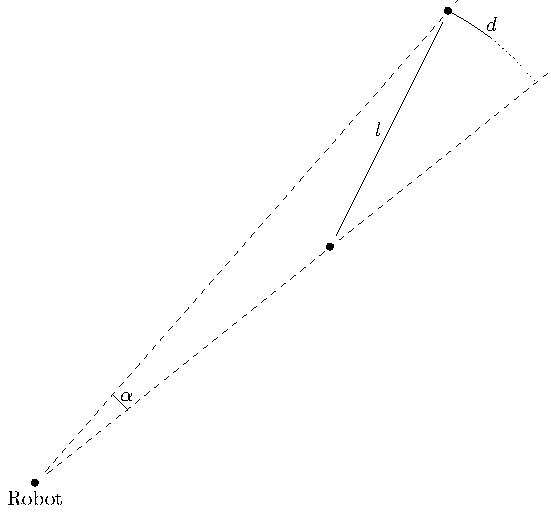
\includegraphics[width=0.4\textwidth]{./img/nms.pdf}
		\end{figure}
	\end{frame}

	\subsection{Correzione dei valori}\label{subsec:Correzione-dei-valori}
	\begin{frame}[allowframebreaks]{Correzione dei valori}
		Per migliorare la stima sulla distanza abbiamo paragonato le reali
		distanze dei target con le stime effettuate dal sistema ottenendo il
		polinomio interpolante $0.003116*x^5 - 0.09722*x^4 + 1.124*x^3
		-5.908*x^2 + 14.5*x-7.367$, che approssima la funzione di correzione della stima. 
		
		\begin{figure}[H]
			\centering
			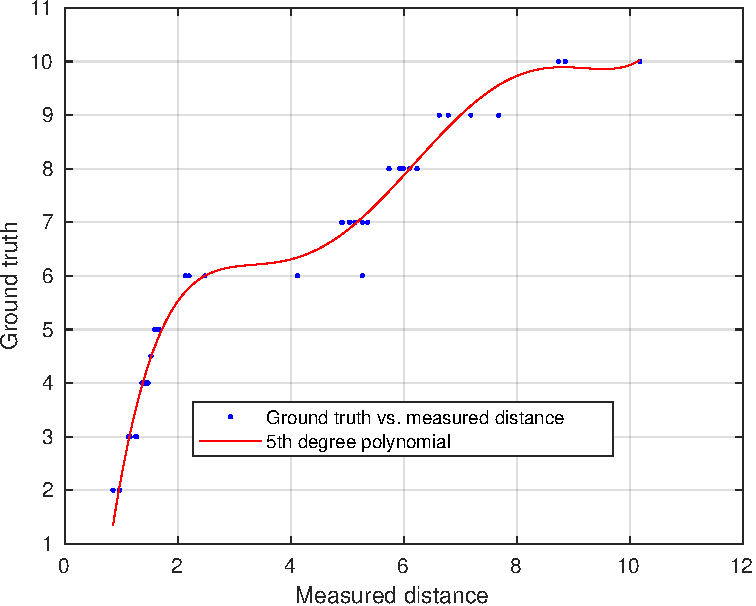
\includegraphics[width=0.6\textwidth]{./img/interpolation.pdf}
			\label{fig:interpolation}
		\end{figure}

	\framebreak
	
	Le bontà della stima della distanza e dell'angolo si evince dalle figure :

	\begin{figure}[ht]
		\begin{subfigure}{.49\textwidth}
			\centering
			% include first image
			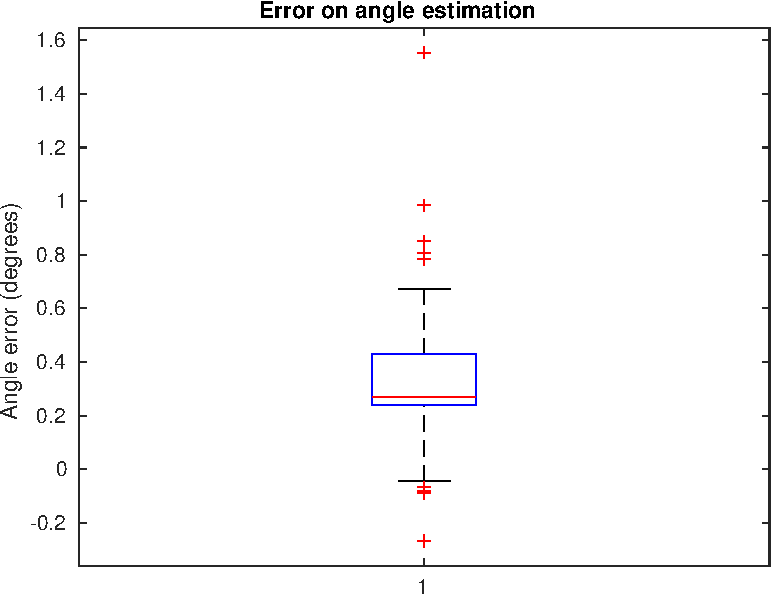
\includegraphics[width=1\linewidth]{./img/angle_error.pdf}  
			\label{fig:angle_plot}
		\end{subfigure}
		\begin{subfigure}{.49\textwidth}
			\centering
			% include second image
			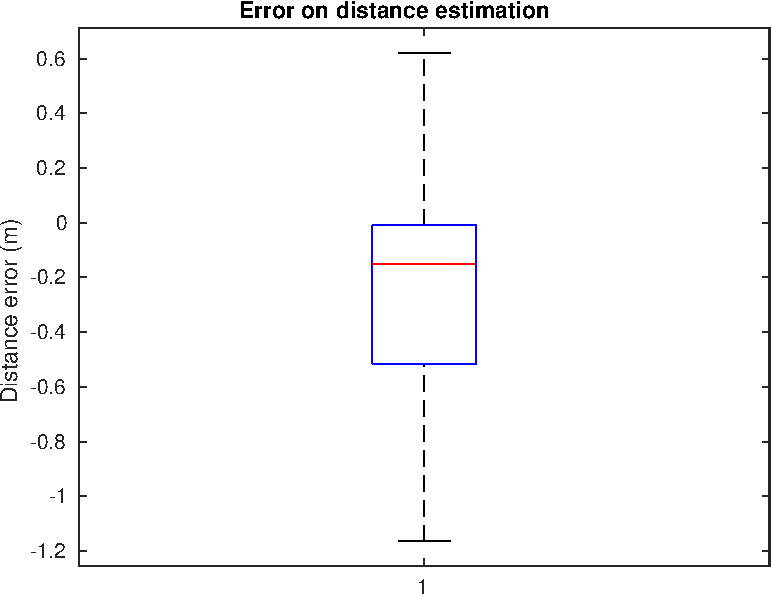
\includegraphics[width=1\linewidth]{./img/distance_error.pdf}  
			\label{fig:distance_plot}
		\end{subfigure}
		\caption{Box plot relativi all'errore su angolo e distanza}
		\label{fig:boxes_plot}
	\end{figure}

	\framebreak

	Nelle figure viene riportata la distribuzione gaussiana multivariata rispettivamente in 3 e 2 dimensioni :
	\begin{figure}[H]
		\begin{subfigure}{0.49\linewidth}
			\centering
			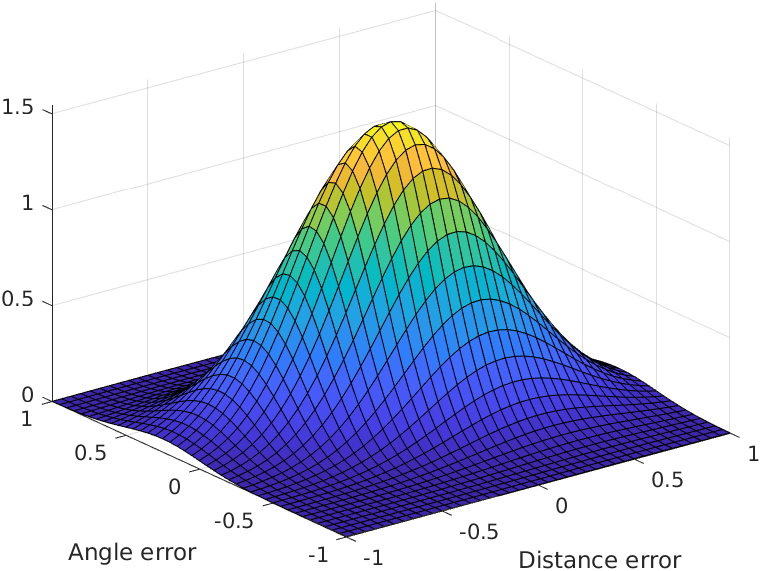
\includegraphics[width=\textwidth]{./img/error_covariance.png}
			\label{fig:error_covariance}
		\end{subfigure}
		\begin{subfigure}{0.49\linewidth}
			\centering
			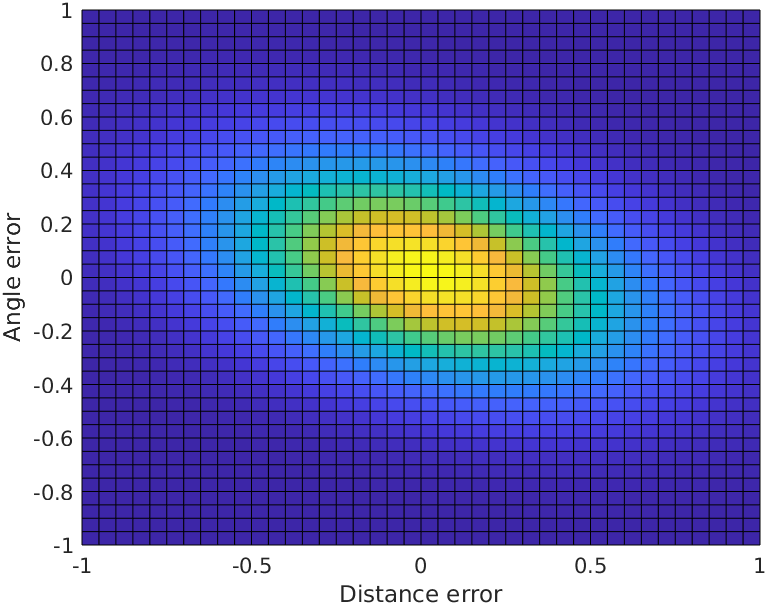
\includegraphics[width=\textwidth]{./img/error_covariance_flat.png}
			\label{fig:error_covariance_flat}
		\end{subfigure}
	\end{figure}

	\end{frame}

	\subsection{Modello probabilistico}\label{subsec:Modello-probabilistico}
	\begin{frame}{Modello probabilistico}
	Nella nostra applicazione la distanza stimata
	dell'oggetto sarà soggetta ad errore non trascurabile. Per questa
	ragione e per i problemi legati alla triangolazione abbiamo abbandonato la
	rappresentazione basata su oggetti e abbiamo fatto ricorso ad un filtro di
	occupazione bayesiano (BOF)~\cite{tay2008bayesian}.
	\end{frame}

	\subsection{Bibliografia}\label{subsec:Bibliografia}
	\begin{frame}{Bibliografia}
		% Bibliography
		\bibliographystyle{unsrt}
		\bibliography{references.bib}.
	\end{frame}

\end{document}
